\documentclass[
tikz,
border=5pt,
convert={density=600,
	outext=.png
}
]{standalone}


\usepackage[utf8]{inputenc}
\usepackage{stanli}
\usepackage{tikz}
\usetikzlibrary{arrows.meta,arrows,positioning,calc,backgrounds}

\begin{document}
	
	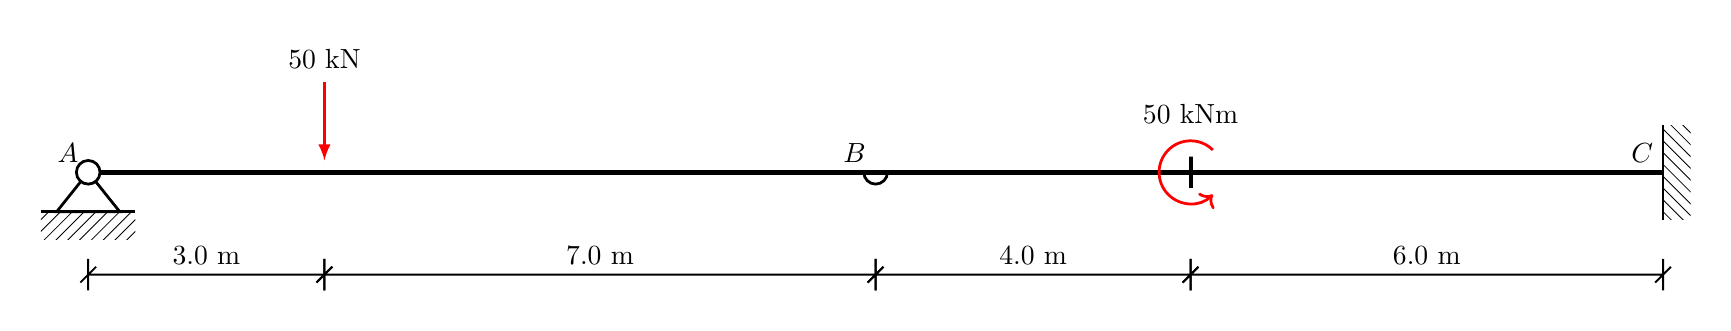
\begin{tikzpicture}[background rectangle/.style={fill=white!45}, show background rectangle]
		
		% Draw beam, supports, notation
		% Stations
		\point{a}{0}{0};
		\point{b}{10.0}{0};
		\point{c}{20.0}{0};
		
		% Midpoints for later reference
		\node(ab) at ($(a)!.3!(b)$) {};
		\node(bc) at ($(b)!.4!(c)$) {};
		
		% Draw the beam between the stations
		\foreach \startn/\endn in {a/b,b/c}
			\beam{4}{\startn}{\endn};
		
		% Supports
		\support{1}{a};
		\support{2ooo}{b};
		\support{3}{c}[90];
		\hinge{2}{b}[a][c];
		
		% hinges
		\foreach \startpt in {a}
			\hinge{1}{\startpt};
		
		% Dimensions
		\dimensioning{1}{a}{ab}{-1.3}[$3.0$~m];
		\dimensioning{1}{ab}{b}{-1.3}[$7.0$~m];
		\dimensioning{1}{b}{bc}{-1.3}[$4.0$~m];
		\dimensioning{1}{bc}{c}{-1.3}[$6.0$~m];
		
		% Letters - no ticks = 1; ticks = 2
		\notation {1}{a}{$A$}[above left];
		\notation {1}{b}{$B$}[above left];
		\notation {1}{c}{$C$}[above left];
		
		\begin{scope}[color=red]
			\load{1}{ab}[90]
			\load{3}{bc}[45]
		\end{scope}
		\notation{2}{bc}{$50$ kNm}[above=5mm];
		\notation{1}{ab}{$50$ kN}[above=12mm];
		
	\end{tikzpicture}
	
\end{document}